% !TEX TS-program = pdflatex

\documentclass[11pt]{amsart}
\usepackage{hyperref}
\usepackage[letterpaper,left=1in,right=1in,top=1in]{geometry}

\usepackage{tikz}
\usetikzlibrary{positioning,chains,fit,shapes,calc,arrows,patterns}
\usepackage{tkz-graph}
\usetikzlibrary{arrows, petri, topaths}
\usepackage{tkz-berge}
\usepackage[all]{xy}
\usepackage{amssymb}


\begin{document}

\begin{center}
\bf Current Problem Sets
\end{center}
\vskip 10 pt

General instructions: Write up the solutions for the problems in each lesson. Scan the work
into a pdf file.  No other file format is accepted. If there are multiple pages for an assignment, merge the pages into a single pdf. 
Upload your work to Blackboard.  Give the file an identifying name such as MyNameMath208L01.pdf
(the L01 is for Lesson 1).
Be sure to save the file with such a name on your computer, not just in Blackboard, since the name of the file
on  your computer will be the name it will have when it is downloaded from Blackboard.  

Make sure the work is dark enough to be read. Use a dark pen or pencil, or
maybe increase the contrast on the scanner.  Show the work that leads to the solution; correct answers without necessary work will earn little if any credit.

 Remember that you cannot expect more than three assignments
to be graded in any seven day period. Graded assignments will be available through Blackboard.

Problems 1 through 5 are worth are worth $5$ points each. Problem 6 is a bonus problem worth $3$ points. The total score for a problem set cannot be greater than $25$.

Sample exercises with solutions are found in an appendix to the text. When solving the problems in this list,
you may use any facts given in the text {\bfseries exercises} \underbar{but not in the text {\bfseries problems}}.
If you want to use a fact in a problem, give a solution to the problem as part of your work. 

\medskip
\begin{center} 
Problems to be submitted.
\end{center}
\medskip



\section{Lesson 1}

\begin{enumerate}


\item Determine which of the following sentences are propositions. Give a brief reason for your answer.
\begin{enumerate} 

\item Seven is two more than five.

\item Stop whining!

\item There is a black hole at the center of every galaxy.

\item This sentence has five words. \\[10pt]

\end{enumerate}


\item Construct truth tables for each of the following.

\begin{enumerate} 

\item$\neg q\longrightarrow p$.

\item $(p\lor q)\longrightarrow  r$. 
(You will need eight rows for this one.)\\[10pt]

\end{enumerate}


\item Let $s$ be the proposition {\itshape It is snowing}, $f$ be the proposition 
{\itshape It is below freezing}, and $r$ be {\itshape It is raining}. Convert the following English sentences into statements
using the symbols $s$, $f$, $r$ and logical connectives.

\begin{enumerate}

\item It is snowing or it is not below freezing.

\item If it is snowing, then it is not raining and it is below freezing.\\[10pt]

\end{enumerate}

\item  Use a truth table to verify  the  equivalence:
$p\longrightarrow \neg q\equiv \neg p\lor\neg q$.\\
Explain why the truth table shows that the propositions are equivalent.\\[10pt]

\item Use a truth table to show that the statements $p\longrightarrow (q\longrightarrow r) \text{ and  }(p\longrightarrow q)\longrightarrow r$ \\
are not logically equivalent. \\
Explain why the truth table shows that the propositions are not equivalent.\\[10pt]


\item ({\bf bonus}) Give a proof of the following equivalence following the pattern
of proof shown in the examples in section 2.6 of the text:  $\neg p\longrightarrow(p\longrightarrow q)\equiv {\bf T}$.\\[10pt]

\end{enumerate}

\section{Lesson 2}

\begin{enumerate}

\item Let $P(x): x^2\leq 4$.  The domain for $x$ is all positive integers ($1,2,3,\ldots$). Determine the truth values of the following propositions. 
\begin{enumerate}
\item $P(5)$
\item$\neg \forall x\, P(x)$\\[5pt]
\end{enumerate}

\item Let $P(x,y)$ be {\it $x$ has read $y$}, where the domain of discourse for 
$x$ is all students
in this class, and the domain of discourse for $y$ is all books written by Mark Twain. Express the
following propositions in English. 
\begin{enumerate}
\item $\forall x\, P(x,\text{Huckleberry Finn}).$
\item $\exists x\, \forall y\, P(x,y).$
\item $\forall y\, \exists x\, P(x,y).$\\[5pt]
\end{enumerate}

\item Let $F(x,y)$ be the statement {\it $x$ trusts $y$}, where the domain of discourse
for both $x$ and $y$ is  all people. 
\begin{enumerate}
\item
 Use quantifiers to express each of the following propositions in symbols.
\begin{enumerate}
\item Nobody trusts Ralph.

\item Everybody trusts Fred.

\item Somebody trusts everybody.

\end{enumerate}

\item Now write the negation of those propositions in symbols. The cheap way would be to simply write $\lnot$ in front of each of the answers to part (a). Don't do that. Use the rules discussed in the text so your answer does not have $\lnot$ occurring to the left of any quantifiers.

\item Express each of those negations in an English sentence.\\[5pt]

\end{enumerate}

\item  Show that {\it $p\longrightarrow q$ and $\neg p,\quad \therefore \neg q$} is not a valid rule
of inference. It is called the fallacy of denying the hypothesis. To expand a bit on the reading for this lesson, here is how to show a proposed rule of inference is valid using a truth table: Construct a truth table with columns for the hypotheses and a column for the conclusion. Check that in every row where the hypotheses all have truth value {\bf T}, the conclusion also has truth value {\bf T}. In plain English, check that if we agree the hypotheses are all true, then the conclusion is true as well. Notice that in rows where the hypotheses do not all have truth value {\bf T}, the truth value of the conclusion does not matter. Flipping that {\it validity test}  around, an argument is not valid if there is a row in the truth table where the hypotheses are all {\bf T}, but the conclusion is {\bf F}. Such a row shows that it is possible to agree that the hypotheses are all true, and yet still have the conclusion false. That means the argument is not valid.\\[5pt]


\item Express the following argument symbolically, and then prove, using the style of proof shown in \underbar{table} 4.2 of the text,  that the argument is valid.  {\it If Ralph doesn't have a sore shoulder
or he doesn't feel sick, then he will go bowling and  he will go to the movie. If he goes to the movie, he will buy popcorn.  He didn't buy popcorn. So Ralph has a sore shoulder.}

(Use
$s$ for Ralph has a sore shoulder.
$f$ for Ralph feels sick. 
$b$ for Ralph goes bowling.
$m$ for Ralph goes to the movie.
$p$ for Ralph buys popcorn.

Warning: You will probably want to use the rule of Simplification at some point in your proof. You need to be careful with that rule! In plain English, the rule says that if you know $p$ and $q$ is true, then you can conclude $p$ is true. But watch out: if $p \land q$ is part of a larger proposition, you can not replace $p \land q$ with $p$. For example, consider the proposition {\it If I bet \$1000 on My Pony and My Pony wins the race, then I will be rich.} Obviously it is not valid to say, by Simplification, {\it If I bet \$1000 on My Pony, then I will be rich.} So, be careful using Simplification.\\[5pt]


\item (bonus) Prove
\begin{align*}
&\exists{x}(A(x)\land\neg B(x))\\[4pt]
&\forall{x}(A(x) \longrightarrow C(x))\\[4pt]
\noalign{\kern -10pt}
&\vrule width 1.2truein height 0pt depth .4pt\\[4pt] 
&\therefore \exists{x}(C(x)\land \neg B(x))\\[4pt]
\end{align*}
Hint: This is very similar to example 4.2 in the text.\\[5pt]

\end{enumerate}


\section{Lesson 3}

\begin{enumerate}


\item Write the following sets using the roster form:

\begin{enumerate}
\item $\{x \in \mathbb{Z} | 10\leq x^2< 100\}$ (Careful, that is $\mathbb Z$, not $\mathbb N$!)
\item  $\{x\in \mathbb{N} | x\leq 4\}$ (Remember that, in this text anyhow, $0\in \mathbb{N}$.)\\[3pt]
\end{enumerate}

\item Use set-builder notation to give a description of each set.
\begin{enumerate}
\item $\{ 4, 8, 12\}.$
\item $\{-2, 0, 2, 4, 6\}.$\\[3pt]
\end{enumerate}

\item  Let $A=\{1,2,3,5,6,7\}$ and $B=\{2,4,6,8,9\}$. Find 
\begin{enumerate}
\item $A\cap B$
\item $A\cup B$
\item $A-B$
\item $B-A$\\[3pt]
\end{enumerate}

\item Draw Venn diagrams for $A\cap (B \cup C)$ and $(A\cap B)\cup(A\cap C)$ to  show that $A\cap (B \cup C) = (A\cap B)\cup(A\cap C)$.\\[3pt]


\item Let $A=\{1,2,3,4\}\times\{1,2,3\}$. List the elements of the set
$B= \{ (s,t)\in A\,|\, s\geq t\,\}$.\\[3pt] 

\item (bonus) Is the proposition {\it Every element of the empty set has 
three toes} true or false? Explain your answer! Hint: In symbols, the proposition is written:
  $\forall x (x\in \emptyset \longrightarrow x \text{ has three toes})$. Think about the truth value of that implication.

\end{enumerate}

\section{Lesson 4}

\begin{enumerate}

\item [] For  these exercises, you will need to know the definitions of even and odd integers. 
 An integer $n$ is {\it even} if $n=2k$ for some integer $k$. An integer $n$ is {\it odd}
if $n=2k+1$ for some integer $k$. There are no integers that are both even and odd!
Examples: $6$ is even since $6 = (2)(3)$, $-8$ is even since $-8 = (2)(-4)$, $0$ is even since $0 = (2)(0)$, $3$ is odd since $3 = 2(1)+1$, and $-9$ is odd since $-9 = (2)(-5)+1$.\\[8pt]


\item Give a direct proof that the sum of  an odd integer and an even integer is odd. 

Hint: Start by letting $m$ be an odd integer and letting $n$ be an even integer. That means $m = 2k+1$ for some integer $k$ and $n = 2j$ for some integer $j$. Notice that if we let the odd and even integers be $2k+1$ and $2k$, the proof will only account for the cases in which $n$ is one less than $m$.
That is why we need to have $m = 2k+1$ and $n=2j$ for integers $k,j$, so that the sum of  any odd and any even will be considered. 
You are interested in $m+ n$, so add them up and see what you get.  Why is the thing you get an odd integer (think about the definition of {\it odd})?\\[5pt]

\item Give an  indirect proof that if $n^3$ is even, then $n$ is even. Hint: Study the solution of a similar statement in the sample solutions for this lesson.\\[5pt]


\item Give a proof by contradiction that if $5n-4$ is odd, then $n$ is odd.

Hint:  This is the problem in this set that gives the most grief.  Study the section
in  the  notes  where  the  mechanics  of  proving  a  statement  of  the  form
If P, then Q by contradiction is discussed.  Be sure you understand why the first line of the proof should be something like {\it Suppose $5n- 4$ is odd {\bfseries and} $n$ is even.}\\[5pt]

\item  Give an example of a predicate $P(n)$ about positive integers $n$, such that
$P(n)$ is true for every positive integer from 1 to one billion, but which is never-the-less not
true for all positive integers.  (Hints:  (1) There is a really simple choice possible for the predicate
$P(n)$, (2) Make sure you write down a {\bfseries predicate} with variable $n$, and not a {\bf proposition}!)
The purpose of this problem is to convince you that when checking a
{\it for all}
type proposition, it is not good enough to just check the truth for a few sample cases,
or, for that matter, even a few billion sample cases.  A general proof that covers all
possible cases is necessary.\\[5pt]

\item Give a counterexample to the proposition {\it Every positive
integer that ends with the digits $13$ is a prime.}\\[5pt]

\item(bonus) 
The {\bfseries maximum} of two numbers, $a$ and $b$, is $a$ provided $a\geq b$. Notation: $\max(a,b) = a$. The {\bfseries minimum}
of $a$ and $b$ is $a$ provided $a\leq b$. Notation: $\min(a,b) = a$.  Examples: $\max(2,3) = 3$, $\max(5,0) = 5$, $\min(2,3) = 2$,
$\min(5,0) = 0$, $\max(4,4) = \min(4,4) = 4$.\\
Give a proof by cases (two cases is the natural choice for this problem)  that for any numbers $s,t$,
\[\min(s,t)+\max(s,t) = s+t.\]\\[5pt]
\end{enumerate}

\section{Lesson 5}

\begin{enumerate}

\item  Let $A=\{a,b,c,d\}$ and $R=\{(a,a),(a,c), (b,b), (b,d),(c,a),(c,c)\}$ be a relation
on $A$. Draw a digraph which represents $R$. You might want to review the definition of digraph!\\[5pt]


\item Find the composition, $R\circ S$,  where $S = \{\,(1,a), (4,a),
(5,b), (2,c),  (3,c), (3,d)\,\}$ with $R  =\{(a,x),(a,y),(b,x),(c,z),(d,z)\}$ as a set of ordered pairs.\\[5pt]

\item Let $R_1=\{(1,2), (1,3), (1,5), (2,1), (5,6), (6,6)\}$ and\\
$R_2=\{(1,2),(1,6), (3,6), (4,2), (5,6), (6,2), (6,3)\}$. Find $R_1\cup R_2$ and $R_1\cap R_2$. \\[5pt]

\item Define a relation on $\{1,2,3,4,5\}$ by $R=\{(1,2),(2,1),(2,3),(3,2),(3,4),(4,3),\\
(4,5),(5,4),(5,1),(1,5)\}$. For each of the five properties of a relation defined in this chapter 
(reflexive, irreflexive, symmetric, antisymmetric, and transitive) 
either show $R$ satisfies the property, or explain why it does not.
\\[5pt]

\item Define the relation {\it $M(A,B) : A\cap B \not= \emptyset$}, where the
domains for $A$ and $B$ are all subsets of $\mathbb{Z}$. For each of the five properties of a 
relation defined in this chapter (reflexive, irreflexive, symmetric, antisymmetric, and transitive) 
either show $M$ satisfies the property, or explain why it does not.
\vskip 4pt
Hint: This problem causes a lot of grief. The relation $M$ is a relation between \underbar{subsets} 
of $\mathbb{Z}$. For example, $\{1,2\} M \{ 9\}$ is false, since $\{1,2\}\cap \{9\} = \emptyset$. But 
$\{1,2\} M \{2,4,6,7\}$ is true since $\{1,2\} \cap \{2,4,6,7\} = \{2\}$, and not $\emptyset$.\\[5pt]

\item (bonus)  Let $A=\emptyset$ and consider the empty relation, $E=\emptyset$,  on $A$. 
For each of the five properties of a 
relation defined in this chapter (reflexive, irreflexive, symmetric, antisymmetric, and transitive) 
either show $M$ satisfies the property, or explain why it does not.

\underbar{Warning}: Reasoning about the empty set can cause grave mental anguish. Suggestion: write out each of the
five definitions you need to check (reflexive, symmetric, etc.) and decide if the statement is true or false.

For example: For the reflexive condition, the statement to check is

\[
\forall x ( x\in \emptyset \implies (x,x)\in E)
\]

Since the left side of the implication ($x\in \emptyset$) is definitely false (after all there isn't anything in the empty set!)
the entire implication is true (recall the truth table for implication). That means the proposition above is true, and so $E$ is reflexive. Reasoning for the remaining four conditions all follow a similar pattern.\\[5pt]

 \end{enumerate}

\section{Lesson 6}

\begin{enumerate}

\item Let $A$ be the set of people alive on earth. 
For each relation defined below, determine if
it is an equivalence relation on $A$. {\bf If it is, describe the equivalence classes.}
If it is not, determine which properties of an equivalence relation fail.\\[3pt]

\begin{enumerate}

\item $a\,H\,b \iff$  $a$ and $b$ are the same age in (in years).\\[3pt]

\item $a\,G\,b \iff$  $a$ and $b$ have at least one grandparent in common.\\[5pt]

\end{enumerate}

\item Consider the relation {\it $S(x,y) : x$ is a brother or sister of $y$} on the set, $H$,
of living humans. (For the purposes of this problem, {\itshape a sibling} of a person means another person  with the same two parents, so don't consider {\itshape half siblings}.) Determine which of the three properties, reflexive, symmetric, transitive,
hold for the relation $S$ (explain your three answers). (Hint: Think carefully about transitive! Almost everyone gets this part wrong.) 
Is $S$ an  equivalence relation on $H$?\\[5pt]

\item  There are many different equivalence relation possible on the set $A=\{a,b,c,d\}$. For example,
here are just three different ones:\\[3pt]
\begin{enumerate} 
\item$E_{1} = \{(a,a), (b,b), (c,c), (d,d), (a,c), (c,a),(b,d),(d,b)\}.$\\[3pt]
\item$E_{2} = \{(a,a), (b,b), (c,c), (d,d), (a,c), (c,a),(a,b),(b,a),(b,c),(c,b)\}.$\\[3pt]
\item $E_{3} = \{(a,a), (b,b), (c,c), (d,d)\}.$\\[3pt]
\end{enumerate}

$E_{1}$ has $8$ ordered pairs while $E_{2}$ has $10$ and $E_{3}$ has $4$. Question: Of all the possible equivalence relations on $A$, what is the largest number of ordered pairs possible in the relation?\\[5pt]



\item Let $A$ be the set of all ordered pairs of positive integers.
So some members of $A$ are $(3,6),  (7,7), (11,4), (1,2981)$. A relation on $A$ is defined by the rule 
$(a,b) R (c,d)$ if and only if $ad = bc$. For example $(3,5) R (6,10)$ is true since $(3)(10)=(5)(6)$.\\[3pt]
\begin{enumerate}
\item Explain why $R$ is an equivalence relation on $A$.\\[3pt]
\item List four ordered pairs in the equivalence class of $(2,3)$.\\[5pt] 
\end{enumerate}

\item   Let $A=\{1,2,3,4,5,6\}$. 
 The sets $\{1, 2\}, \{3, 4, 5\}$, and $\{6\}$ form a partition of $A$.
These are the equivalence classes for an equivalence relation, $E$, on $A$.
 Draw the  {\bf digraph} of $E$.\\[5pt]

\item (bonus) Let $A = \{ 1,2,3\}$. The relation $E = \{ (1,1),(2,2),(3,3),(2,3),(3,2)\}$ is an
equivalence relation on $A$.  $F=\{ (1,1),(2,2),(3,3),(1,2),(2,1)\}$ 
is another equivalence relation on $A$. Compute the composition $F\circ E$.
Is $F\circ E$ and equivalence relation on $A$?

\end{enumerate}

\section{Lesson 7: Test \#1}

\section{Lesson 8}

\begin{enumerate}

\item  What is the $50^{th}$ term of the arithmetic sequence with initial
term $4$ and common\\
 difference $3$?\\[5pt]


\item Evaluate $\displaystyle\sum_{k=-3}^{4} (2k+5)$. (Hint: Since there are only eight terms in the sum, you can just write
them all out and add.)\\[5pt]

\item   Evaluate $\displaystyle \sum_{i=0}^{99} \left(-\frac{2}{3}\right)^i$. (Hint: Since there are $100$ terms in the sum, it isn't a good idea to write them all out and add. Use the formula for the sum of terms of a geometric sequence. Leave the answer with exponents rather than using a calculator to try to get a decimal approximation of the answer.) \\[5pt]

\item 
\begin{enumerate}

\item List the first four terms of the sequence defined recursively by
 $a_0 = 2$, and, for $n\geq 1$, $a_n = 2a_{n-1}^2 -1$.\\[3pt]

\item List the first five terms of the sequence with initial terms
$u_1=1$ and $u_2=5$, and, for $n\geq 3$, $u_n = 5u_{n-1}-6u_{n-2}$.
Guess a closed form formula for the sequence.
Hint: The terms
are simple combinations of powers of $2$ and powers of $3$.\\[5pt]

\end{enumerate}

\item  Give a {\bf recursive} definition of the geometric sequence
with initial term $a$ and common\\
 ratio $r$. 

Hint: $a_{n} = a r^{n-1}$ isn't a correct answer since this formula isn't recursive.
Make sure you write down a recursive formula: (1) give the initial term, and 
(2) give the rule for building new terms from previous terms.\\[5pt]

\item (bonus) Express in summation notation: $\displaystyle  \frac{1}{1}+\frac{1}{3}+\frac{1}{5}+
\cdots+\frac{1}{2n-1}$, the sum of the reciprocals of the first $n$ odd
positive integers. (Note that there are $n$ terms in the sum.)

Hint: A common mistake on this question is using the symbol $n$ both as an index for summation
and to indicate the last term to be added in. To make sure you haven't fallen into that trap, replace every
$n$ in your formula by a specific value, say $5$. The result should be a sum
  $\displaystyle  \frac{1}{1}+\frac{1}{3}+\frac{1}{5}+\frac{1}{7}+\frac{1}{9}$.

 \end{enumerate}
 
 \section{Lesson 9}
 
 \begin{enumerate}
 
 \item A set $S$ of integers is defined recursively by the rules: \\[2pt]
 (1) $1\in S$, and (2) If $n\in S$, then
 $2n+1 \in S$. \\[2pt]
 
 \begin{enumerate} 
 \item Is $20\in S$?\\[2pt]
 \item Is $175\in S$?\\[2pt]
 \end{enumerate}
 Explain your answers.\\[5pt]
 
 \item A set, $S$, of strings over the alphabet 
$\Sigma = \{a,b,c\}$ is defined recursively by (1) $a \in S$
and (2) if $x\in S$ then $xbc\in S$. List all the strings in $S$ of length seven or less.\\[5pt]


\item A set, $S$, of positive integers is defined recursively by the rule:\\[2pt]
(1) $3\in S$, and (2) If $n\in S$, then $2n-3\in S$. List {\bfseries all} the elements in the set $S$.\\[5pt]
 
 \item Give a recursive definition of the set of positive integers that end with the digit $7$.\\[5pt]

 
\item Describe the strings in the set $S$ of strings over the alphabet 
$\Sigma = \{a,b,c\}$ defined recursively by (1) $ c \in S$
and (2) if $x\in S$ then $xa\in S$ and $xb\in S$ and $cx\in S$.\\[5pt]

Hint: Your description should be a sentence that provides an easy test to check if a given string
is in the set or not. An example of such a description is: {\it $S$ consists of all strings of $a$'s, $b$'s, and $c$'s,
with more $a$'s than $b$}'s. That isn't a correct description since $cab$ is in $S$ and doesn't have more $a$'s than
$b$'s, and also $baac$ isn't in $S$, but does have more $a$'s than $b$'s. So that attempted description is really 
terrible. The best way to do this problem is to use the rules to build a bunch of strings in $S$ until a suitable
description becomes obvious.\\[5pt]

\item (bonus)  A set $S$ of ordered pairs of integers is defined recursively
by (1) $(1,2)\in S$  and $(2,1)\in S$,  and (2) if $(m,n)\in S$, then $(m+2,n)\in S$, and
$(m,n+2)\in S$, and $(m+1,n+1)\in S$. There is a simple description
of the ordered pairs in $S$. What is it?  Your description should be good enough so that 
you can instantly decide if $(12236, 912242)$ is in $S$. \\[5pt]


\end{enumerate}

\section{Lesson 10}

\begin{enumerate}

\item[]
{\small {\bf Warning}: It's not unusual to find these problems really tough. One difficulty is that these problems will make some demands on your algebra skills. Another difficulty is just getting the format of an inductive proof correct.  Here are a few suggestions concerning that: (1)
Be sure to check the basis case; (2) At the start of the inductive step, clearly state the inductive hypothesis;
(3) After stating the inductive hypothesis, write down what you need to prove; (4) Point out clearly where you
apply the inductive hypothesis in the proof of the inductive step.}\\[3pt] 


\item Use induction to prove: For every integer $n\geq 1$,
\[
1\cdot 2+ 2\cdot 3+3\cdot4+\cdots+n(n+1) = \frac{n(n+1)(n+2)}{3}.\\[5pt]
\]

\item  Use the first form of induction (see example 16.5) to show that using only $4 c\kern -5pt/$ stamps and  $7c\kern -5pt/$ stamps,
any postage amount $18c\kern -5pt/$ or greater can be formed.\\[5pt]

\item  Redo the previous problem using the second form of induction (see example in the text). The basis step is just a bit messier this time, but the inductive step is much easier.\\[5pt]

\item A sequence is defined recursively by the rules: (1) $a_{0} = 0$, and (2) for $n\geq 1$, $a_{n}= 2a_{n-1}+ 2$. Use induction to prove $a_{n}= 2^{n+1}-2$ for all $n\geq 0$.\\[5pt]

\item Use induction to prove: For every integer $n\geq 1$, the number $n^5-n$ is a multiple of $5$.

Hint: An integer is a multiple of $5$ if it is $5$ times some integer. For example,
$165 = (5)(33)$ so $165$ is a multiple of $5$.\\[5pt]

\item   (bonus) Here is a {\itshape proof} that for $n\geq 0$,  $1+ 2 + 2^2 +  \cdots + 2^n = 2^{n+1}$.
\begin{proof}
Suppose $1+ 2 + 2^2 +  \cdots + 2^n = 2^{n+1}$ for some $n\geq 0$. Then
\begin{align*}
 1+ 2 &+ 2^2 +  \cdots + 2^n  + 2^{n+1} = 2^{n+1} +2^{n+1} \qquad\text{using the inductive hypothesis}\\
 &= 2(2^{n+1}) = 2^{n+2} = 2^{(n+1)+1},
 \end{align*}
 as we needed to show.
 \end{proof}
 
 Now, obviously there is something wrong with this proof by induction since, for example,
 $1+2+2^2 = 7$, but $2^{2+1} = 2^3 = 8$. What specifically is wrong with the proof?


\end{enumerate}

\section{Lesson 11}

\begin{enumerate}

\item[]
{\small For the proofs requested below, use facts and theorem 
given in this lesson, including results given in the exercises,  as justifications. Assume all letters represent
integers.}\\[5pt]

\item  Mimic the proof given in the sample solutions for the proposition
 {\it if $a>0$ and $b>0$, then $ab>0$} to prove:\\[3pt]
 
\begin{enumerate}
\item If $a<0$ and $b<0$, then $ab>0$.\\[3pt]
\item If $a<0$ and $b>0$, then $ab<0$.\\[5pt]
\end{enumerate}


\item 
Prove that if $m^{2} = n^{2}$, then $m=n$ or $m = -n$.\\
 (Hints: (1) From algebra: $a^{2}-b^{2} = (a+b)(a-b)$, and \\
 (2) From exercises: If $ab=0$, then either $a=0$ or $b=0$.) \\[5pt]

\item  Determine all the integers that $0$ divides.

Hint: Think carefully about the {\bf definition} of the {\it divides} relation! This question is about the divides relation, not about the arithmetic operation of division (a maybe subtle distinction). The correct answer is probably not what you might first think it is.\\[5pt]


\item Prove: For integers $r,s,t$,and $u$, if $r|t$ and $s|u$, then $rs|tu$.\\[5pt]

\item Determine the quotient and remainder when $117653$ is
divided by $27869$. (Finally, an easy problem.)\\[5pt]

\item (bonus) Prove or give a counterexample: If $p$ is a prime, then $6p+1$ is a prime.\\[5pt]
\end{enumerate}


\section{Lesson 12}

\begin{enumerate}

\item Use the Euclidean Algorithm to compute the following gcd's:\\[3pt]
 \begin{enumerate}
 \item $\gcd(216,111)$.\\[3pt]
 \item $\gcd(1001,11)$.\\[3pt]
 \item $\gcd(663,5168)$.\\[3pt]
 \item $\gcd(1357,2468)$.\\[3pt]
 \item $\gcd(733103,91637)$.\\[5pt]
 \end{enumerate}
 
 
\item  If $p$ is a prime, and $n$ is any integer, what are the
possible values of $gcd(p,n)$?
Hint: Try a few experiments with specific numbers to spot the correct answer. Alternatively, think about the positive integers that can divide a prime. Warning: In the notation $\gcd(a,b)$, do not assume that $a\geq b$.
The two parameters $a$ and $b$ can be written in either order: $\gcd(15,12) = \gcd(12,15) = 3$.\\[5pt]

\item Determine $gcd(6123,2913)$ and write it as a linear combination of $6123$ and $2913$. \\[5pt]

\item What can you conclude about $\gcd(a,b)$ if there are integers $s,t$ such that $as+bt = 8$?\\[5pt]

\item What is the smallest positive integer that can be written as a linear combination of $2191$ and  $1351$?\\[5pt]


\item (bonus) If $n$ is a positive integer, what is $\gcd(n,n+1)$? Explain your answer.


\end{enumerate}

\section{Lesson 13}

\begin{enumerate}

\item Determine the prime factorization of $212100$.\\[5pt]

\item How many positive divisors does $212100$ have?
You don't have to list them all, just determine how many there are. This isn't
difficult using the result of problem 1. See a similar example in the notes. \\[5pt]


\item  Find all integer solutions to $14x+ 77y = 69$.\\[5pt]

\item Find all integer solutions to $14x+ 77y = 70$.\\[5pt]



\item Beth stocked her video store with a number of video game 
machines at \$79 each, and a number of video games at \$41 each.
If she spent a total of \$6358, how many of each item did she purchase?\\[5pt]

\item (bonus) Determine all integer solutions to $5x - 7y = 99$. Watch that minus sign!\\[5pt]

\end{enumerate}

\section{Lesson 14: Test \#2}

\section{Lesson 15}

\begin{enumerate}

\item
\begin{enumerate}
\item Suppose we have a $52$ card deck with the cards in order $\text{ace }, 2, 3, \ldots,\text{ queen, king}$ 
top to bottom, for clubs, then diamonds, then hearts, then spades. A step consists to taking the top card and moving it to the bottom of the deck. We start with the ace of clubs as the top card. After two steps, the top card is the $3$ of clubs. What is the top card after $735$ steps?\\[3pt]

\item The marks on a combination lock are numbered $0$ to $39$. If the lock is at  mark $19$, and the dial is turned one mark clockwise, it will be
at mark $18$. If the lock is at mark $19$ and turned $137$ marks clockwise, at what mark will it be?
\\[5pt]
\end{enumerate}

\item 
\begin{enumerate}
\item Arrange the numbers $-39, -27, -8, 11, 37, 68, 91$ \\
so they are in the order $0,1,2,3,4,5,6$ modulo $7$.\\[5pt]
\item  Determine $n$ between $0$ and $16$ such that\\
 $311+891 \equiv n \,(\bmod\,17)$.\\[3pt]
 \item Determine $n$ between $0$ and $16$ such that \\
$(405)(777) \equiv n \,(\bmod\,17)$.\\[3pt]
\item Determine $n$ between $0$ and $16$ such that\\
 $710^{447} \equiv n \,(\bmod\,17)$.\\[5pt]
\end{enumerate}

\item Find all solutions: $33x\equiv 183\,(\bmod\,753 )$. \\[5pt]

\item  A multiple choice test contains 10 questions. There are four possible answers
for each question.\\[3pt]
\begin{enumerate}
\item How many ways can a student complete the test if every question 
must be answered?\\[3pt]
\item How many ways can a student complete the test if questions 
can be left unanswered?\\[5pt]
\end{enumerate}

\item Here are two questions most easily done using the $\it Good = Total - Bad$ method.\\[3pt]
\begin{enumerate}
\item How many seven-letter words contain at least one $X$?\\[3pt]
\item How many seven-letter words contain at least two $X$'s?
Hint: The {\it Bad} ones are those with no $X$'s and those with exactly one $X$. 
Think carefully about counting the number of words with exactly one $X$.\\[5pt]
\end{enumerate}

\item (bonus) A code word is either a sequence of three letters followed
by two digits or two letters followed by three digits. (Unless otherwise
indicated, {\it letters} will means
 letters chosen from the usual
$26$-letter alphabet and {\it digits} are selected from 
$\{0,1,2,3,\dots,8,9\}$. Also, unless it is stated that letters have to be different, you should assume repeats are allowed. Likewise for digits.) How many different code words are possible?\\[5pt]



\end{enumerate}

\section{Lesson 16}

\begin{enumerate}


\item 
\begin{enumerate}
\item (a permutation problem, order matters) An ID code consists of $4$ \underbar{different} letters and $3$ \underbar{different} digits. How many codes are possible if the letters must be kept together? For example, $34ABCD9$
and $WAXT604$ are good, but $TR67YZ3$ is bad.\\[3pt]
\item (a combination problem, order does not matter) A lottery ticket consists of four different integers between $1$ and $99$ (inclusive). How many different lottery tickets are there?\\[5pt]
\end{enumerate}

\item Determine the coefficient of  $x^4y^5$ in the expansion of $(3x-2y)^9$. Be sure to 
take the $3$ and the $-2$ coefficients into account.\\[5pt]

\item    Give an algebraic proof that $\displaystyle {{2n}\choose 2} = 2{n\choose 2} + n^2$.\\[3pt]
Hint: The idea is to expand and simplify each side of the equation, then compare the two results and make sure they are the same. This problem seems to cause a lot of anguish. It might help if the two sides are computed for a few specific values of $n$ to see how the arithmetic works out. Try $n = 3$ and $n=4$ for example.\\[5pt]

\item A poker hand consists of five cards selected from a $52$ card deck. The order of the cards in a poker hand does not matter. A poker hand is called a {\it full house} if it has two cards of one rank and three cards of a second rank. For example, a hand consisting of two $7$'s and three $queens$ is a full house. How many different full house hands are there?\\[5pt] 

\item How many permutations of the letters {\it a,b,c,d,e,f,g} either begin with an {\it a} or end with an {\it a}?\\[5pt]


\item (bonus) A committee of size five is selected from a group of ten clowns and
twelve  lion tamers.\\[3pt]

\begin{enumerate}
\item How many different committees are possible?\\[3pt]

\item How many committees are possible if there must be exactly two clowns
on the committee?\\[3pt]

\item How many committees are possible if lion tamers must outnumber clowns
on the committee?\\[5pt]

\end{enumerate}

\end{enumerate}

\section{Lesson 17}

\begin{enumerate}

\item Inclusion{-}exclusion counting: Among the members of a book club,
 $20$ people have read {\itshape War and Peace (WP)}, $14$ have read
{\itshape Moby Dick (MD)} and  $27$ have read {\itshape The Great Gatsby (GG)}, $5$ have read WP and GG, $3$ have read MD and GG, $6$ have read WP and MD, and $2$ have read all three books. Assuming everyone in the club has read at least one of those three books, how many members does the book club have?  \\[5pt]

\item  More inclusion{-}exclusion counting: How many bit strings of length $15$ have bits $1,2$, and $3$  equal to $101$, or have bits $12,13,14$, and $15$ equal to $1001$ or
have bits $3,4,5$, and $6$ equal to $1010$? (Number bits from left to right. In other words, bit \#1 is the left most bit and bit \#15 is the right most bit.)

Hint: The fact that the third bit appears in two of the required patterns means some special care will be needed to get the count correct.\\[5pt]


\item  Show that there are two different positive powers of $5$ (in other words, $5^{n}$, for positive integers $n$),  that differ by a multiple of $742361$. (Hint: Using the Pigeon Hole Principle, no arithmetic is needed to do this problem.)\\[5pt]

\item Plutonians have three feet. Suppose the Plutonian Vancleef has a box with one hundreds each of red, blue, yellow, green, and white socks. Plutonian etiquette requires that Vancleef wear three socks of the same color.  It's dark, and Vancleef can't see. What is the minimum number of socks Vancleef needs to take from the box to be sure there will be a suitable triplet of socks?\\[5pt]

\item Rocky has $31$ days to prepare for his Discrete Math final. He has decided to do at least one tough problem each day, but no more than
$50$ problems total. Show there must be a sequence of consecutive days in which he does exactly $11$ problems.\\[5pt]

\item (bonus) Here's a pretty hard looking (but really not too hard if done carefully) inclusion{-}exclusion problem. The correct answer is $76$. You job is to show the work that leads to that answer.

How many permutations of the digits $1,2,3,4,5$, have at least one digit in {\it its
own spot}? In other words, a $1$ in the first spot, or a $2$ in the second, etc.
For example, $35241$ is OK since it has a $4$ in the fourth spot, and $14235$ is OK, since
it has a $1$ in the first spot (and also a $5$ in the fifth spot). But $31452$ in no good.
Hint: Let $A_1$ be the set of permutations that have $1$ in the first spot, let $A_2$ be
the set of permutations that $2$ in the second spot, and so on. As a start, notice that $|A_{1}|
= |A_{2}| = |A_{3}| = |A_{4}| = |A_{5}| = 4!$ \\[5pt]

\end{enumerate}

\section{Lesson 18}

\begin{enumerate}

\item     Suppose on December $31$, $2000$, a deposit of $\$100$ is made in a savings 
account that pays $10\%$ annual interest (Ah, those were the days!). 
So one year after the initial deposit, on  December $31$, $2001$, the account
will be credited with $\$10$, and have a value of $\$110$. On  December $31$, $2002$
that account will be credited with an additional $\$11$, and have value $\$121$.
Find a \underbar{\bf recursive relation} that gives the value of the account $n$ years after the
initial deposit.\\[5pt]

\item Sal climbs stairs by taking either one, two, or three steps at a time.\\[3pt]
  \begin{enumerate}
\item Determine a recursive formula for the number of different ways Sal can climb a
flight of $n$ steps. Don't forget to include the initial conditions. \\[3pt]

\item In how many different ways can Sal climb a flight of ten steps?\\[5pt]
\end{enumerate}

\item  Passwords for a certain computer system are strings of uppercase letters.
A valid password must contain an even number of $X$'s. Determine a recurrence
relation for the number of valid passwords of length $n$.
Note: $0$ is an even number, so $ABBC$ is a valid password. This counting problem is pretty tricky. Here's a good way to think about it: to make a good password of length $n$
you can either (a) add any non-X to the end of a  good password of length $n-1$, or (b) add an X to the end of a {\it bad} password of length $n-1$. For (b) you can use the {\it Good = Total-Bad} trick to count the number of bad passwords of length $n-1$.\\[5pt]
 
 \item  Solve by unfolding: $a_0 = 3$, and, for $n\geq 1$, $a_n = 5a_{n-1}$.\\[5pt]


\item  Solve by unfolding:  $a_0 = 3$, and, for $n\geq 1$,  $a_n = 5a_{n-1}+ 3$.
Hint: This one will involve applying the  geometric sum formula.\\[5pt]


\item (bonus) Suppose the Tower of Hanoi rules are changed so that stones may only be transferred
to an adjacent clearing in one move. Let $I_n$ be  the minimum number of moves required 
to transfer tower from clearing $A$ to clearing $C$? 
For example, it takes two moves to move a one stone tower from $A$ to $C$: One move from $A$ to $B$, then a second move from $B$ to $C$. So $I_1 = 2$\\[3pt]

\begin{enumerate}
\item  By brute force, determine  $I_2,$ and $I_3$. \\[3pt]
 
\item Find a recursive relation for $I_n$.\\[3pt]

\item \underbar{Guess} a formula for $I_n$.\\[5pt]

\end{enumerate}

\end{enumerate}

\section{Lesson 19}

\begin{enumerate}

\item[] 
\begin{center}
{\small Warning: These problems are going to severely tax your algebra skills and maybe also your patience since they are likely to require a lot of time and paper. Be prepared to review some college algebra techniques if necessary.}\\[5pt]
\end{center}

\item Solve $a_0=1$, and $a_n=3a_{n-1},$ for $n\geq 1$ using the characteristic equation method.\\[5pt]

\item Solve $a_0=1$, and $a_n=3a_{n-1} + 1$ for $n\geq 1$ using the characteristic equation method.\\ Hint: Try $a_{n}= A$, a constant,  to find a particular solution.\\[5pt]


\item    Solve $a_0=1, a_1=3$ and $a_n=a_{n-1}+6a_{n-2},$ for $n\geq 2$.\\[5pt]

\item $a_0=1, a_1=3$ and $a_n=a_{n-1}+6a_{n-2}+1,$ for $n\geq 2$.
Hint:  Use the general solution to the homogeneous problem above, and then
 try $a_n = A$, a constant, to find particular solution.\\[5pt]

\item Solve  $a_0=1, a_1=6$ and $a_n=6a_{n-1}-9a_{n-2}+n,$ for $n\geq 2$.

Hints: (1) Be sure to remember what to do when there are repeated characteristic roots.
(2) Try $a_n = An + B$ for a particular solution.\\[5pt]

\item  (bonus)
Solve $a_0=0, a_1=1$ and $a_n=a_{n-1}+a_{n-2}+2^n$, for $n\geq 2$.

Hints: This one involves a lot more algebra than the problems above. Solving 
the homogeneous problem will involve using the quadratic formula. 
The characteristic roots turn out to be $\displaystyle \frac{1\pm \sqrt{5}}{2}$ (but show the work!). For a particular solution, try 
$a_n = A2^n$. You should find $A=4$ (but show the work!).  Put those two pieces together to write down the general solution 
\[ 
a_n = A\left(\frac{1+\sqrt{5}}{2}\right)^n + B\left(\frac{1-\sqrt{5}}{2}\right)^n + 4(2^n)
\]
and the determine the values for $A$ and $B$ by using the two initial conditions, 
$a_0 = 0$ and $a_1 = 1$. The necessary arithmetic will be somewhat complicated, but not impossible. \\[5pt]

\end{enumerate}


\section{Lesson 20}

\begin{enumerate}

\item Determine the adjacency matrix and the incidence matrix for the graph below.\\[3pt]


 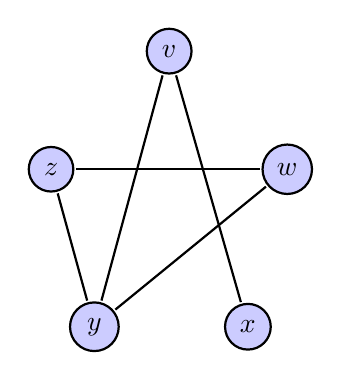
\begin{tikzpicture}[node distance=1cm,
                                 thick,main node/.style={circle,fill=blue!20,draw,outer sep=1pt}
                                ]           
               \node[main node] (1) at (0,0) {$z$};
               \node[main node] (2) at (1.5,1.5) {$v$};
               \node[main node] (3) at (3,0) {$w$};
               \node[main node] (4) at (2.5,-2.00) {$x$};
               \node[main node] (5) at (0.55,-2.00) {$y$};       
            
               \path%
                 (1) edge node [right] {} (3)  %{} is where the edge value would go
                 (3) edge [right] node {} (5)
                 (5) edge [right] node {} (2)
                 (2) edge [left] node {} (4)
                 (5) edge [right] node {} (1);
           \end{tikzpicture}\\[5pt]
           

\item  For the graph below
 \begin{enumerate}
  \item  Find an Eulerian circuit, or prove that none exists.\\[3pt]
  \item  Find a Hamiltonian circuit or prove that none exists.\\[3pt]
 \end{enumerate}
 
 
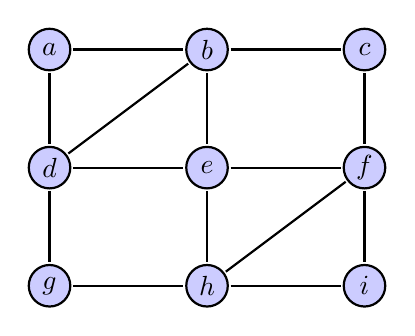
\begin{tikzpicture}[thick,
                       main node/.style={circle,fill=blue!20,draw,outer sep=1pt,
                                         inner sep=1pt,minimum size=15pt}
                      ] 
   \node[main node] (a) at (0.0,3.0) {$a$};
   \node[main node] (b) at (2.0,3.0) {$b$};
   \node[main node] (c) at (4.0,3.0) {$c$};
   \node[main node] (d) at (0.0,1.5) {$d$};
   \node[main node] (e) at (2.0,1.5) {$e$};
   \node[main node] (f) at (4.0,1.5) {$f$};
   \node[main node] (g) at (0.0,0.0) {$g$};
   \node[main node] (h) at (2.0,0.0) {$h$};
   \node[main node] (i) at (4.0,0.0) {$i$};
   \path%
    (a) edge [left] node {} (b)
    (a) edge [left] node {} (d)
    (b) edge [left] node {} (c)
    (b) edge [left] node {} (e)
    (b) edge [left] node {} (d)
    (c) edge [left] node {} (f)
    (d) edge [left] node {} (e)
    (d) edge [left] node {} (g)
    (e) edge [left] node {} (f)
    (e) edge [left] node {} (h)
    (f) edge [left] node {} (h)
    (f) edge [left] node {} (i)
    (g) edge [left] node {} (h)
    (h) edge [left] node {} (i);
  \end{tikzpicture}\\[5pt]
  
 \item  For the graph below
 \begin{enumerate}
  \item  Determine all the bridges.\\[3pt]
  \item  Determine all the cutvertices.\\[3pt]
 \end{enumerate}
 
 
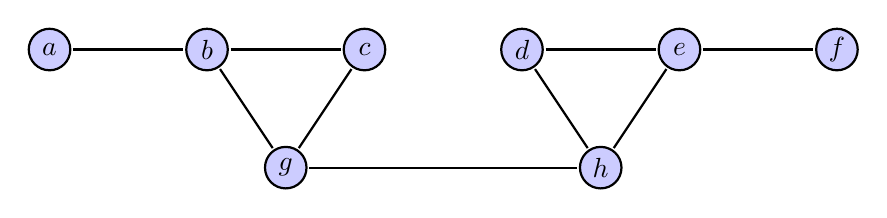
\begin{tikzpicture}[thick,
                       main node/.style={circle,fill=blue!20,draw,outer sep=1pt,
                                         inner sep=1pt,minimum size=15pt}
                      ] 
   \node[main node] (a) at (0.0,3.0) {$a$};
   \node[main node] (b) at (2.0,3.0) {$b$};
   \node[main node] (c) at (4.0,3.0) {$c$};
   \node[main node] (d) at (6.0,3.0) {$d$};
   \node[main node] (e) at (8.0,3.0) {$e$};
   \node[main node] (f) at (10.0,3.0) {$f$};
   \node[main node] (g) at (3.0,1.5) {$g$};
   \node[main node] (h) at (7.0,1.5) {$h$};
   
   \path%
    (a) edge [left] node {} (b)
    (b) edge [left] node {} (c)
    (d) edge [left] node {} (e)
    (e) edge [left] node {} (f)
    (b) edge [left] node {} (g)
    (c) edge [left] node {} (g)
    (d) edge [left] node {} (h)
    (g) edge [left] node {} (h)
    (e) edge [left] node {} (h);
  \end{tikzpicture}\\[5pt]


\item For each candidate degree sequence below, either draw a graph with that degree sequence or explain why that list cannot be the degree sequence of a graph.\\[3pt]

\begin{enumerate}
\item $4,4,4,4,4  $   \\[3pt]
\item $6,4,4,4,4  $   \\[3pt]
\item $0,0,0,0,0  $   \\[3pt]
\item $3,2,1,1,1  $   \\[3pt]
\item $3,3,2,2,1  $   \\[5pt]
\end{enumerate}



\item A {\it forest} is a graph consisting of one or more (separate) trees. If the total number of vertices in a forest is $f$, and the number of trees in the forest is $t$, what is the total number of edges in the forest?\\[5pt] 


\item (bonus) A tree is called {\bf star{-}like} if there is exactly one vertex with degree greater than $2$. How many different (that it, nonisomorphic) star{-}like trees are there with six vertices? (Note: If you draw the graph with the vertex of of degree greater than $2$ having the {\it arms} of the tree radiating out from it like spokes on a wheel, the name star{-}like will make sense.\\[5pt]
\end{enumerate}


\section{Lesson 21: Test \#3}


\end{document}

\bye